\chapter{Background}\label{chap:background}
\begin{figure}[ht]
\centering
     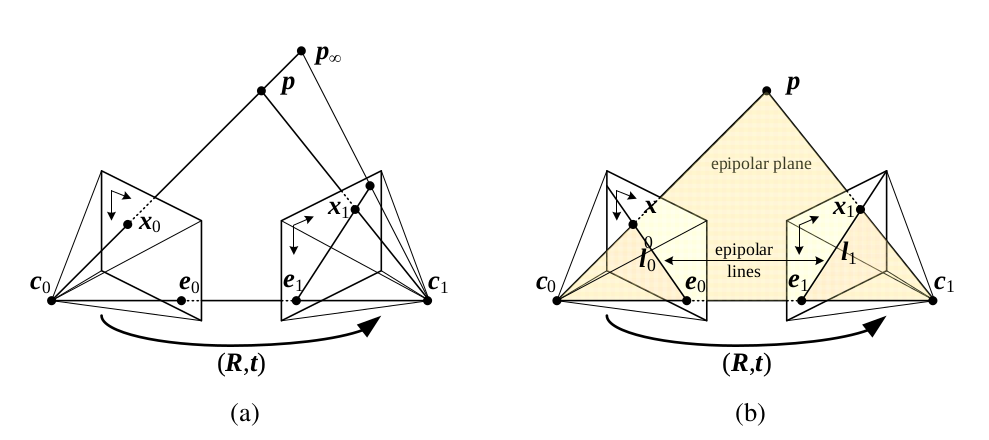
\includegraphics[width=1.0\textwidth]{images/epipolar.png}
      \caption[A typical Epipolar Geometry Setup]{\textbf{A typical Epipolar Geometry Setup.} $\mathbf{p}$ is the 3D point in the scene. $\mathbf{c_0}$ and $\mathbf{c_1}$ are the centers of the cameras. The triangle defined by the points $\mathbf{p,c_0,c_1}$ is the epipolar plane. The line $\mathbf{c_0}$,$\mathbf{c_1}$ that connects the two camera centers is the baseline, and the lines $\mathbf{x_0,e_0}$, and $\mathbf{x_1,e_1}$ are the epipolar lines. This image is obtained from \cite{Szeliski2010book}} 
       \label{fig:epipolar}
\end{figure}

In {\mvs} methodologies, camera matrices, source views, and reference views play crucial roles in establishing correspondences, predicting depth, and, ultimately, the reconstruction process.  There is an interesting relationship between the multiple cameras, the 3D point in the scene, and its projections in the image planes of the cameras. These relationships can be described by epipolar geometry.  \hyperref[fig:epipolar]{Figure 1} shows a standard epipolar geometry setup. This setup involves 2 cameras at $\mathbf{c_0}$ and $\mathbf{c_1}$ observing the same 3D point $\mathbf{p}$ in the scene. $\mathbf{x_0}$ and $\mathbf{x_1}$ are the projections of $\mathbf{p}$ on the image planes of the two cameras.\par 
First, we will define the terminology associated with epipolar geometry and the estimation of the depth/disparity. Then, in the subsequent sections, we will formalize the definitions and draw connections between the different concepts. 

\section{Relevant Terminology}

\begin{itemize}
\item \textbf{Epipolar Plane:} Epipolar plane is the plane defined by the centers of the cameras and a 3D point in the scene. In Figure \hyperref[fig:epipolar]{1}, the triangle defined by the points $\mathbf{p,c_0,c_1}$ is the epipolar plane. 
\item \textbf{Epipolar Line:} The intersections of the epipolar plane with the image planes are known as the epipolar lines. In Figure \hyperref[fig:epipolar]{1}, the two lines $\mathbf{x_0,e_0}$ and $\mathbf{x_1,e_1}$ are the epipolar lines.
\item \textbf{Epipoles:} The points of intersection of the baseline $\mathbf{c_0},\mathbf{c_1}$ with the image planes are the epipoles. In Figure \hyperref[fig:epipolar]{1}, the points $\mathbf{e_0}$ and $\mathbf{e_1}$ are the epipoles. 
\item \textbf{Epipolar Constraint:} It is the fundamental rule of epipolar geometry that states that any projection $\mathbf{x_0}$ of the 3D point $\mathbf{p}$ in one image must lie on the corresponding epipolar line $\mathbf{x_1, e_1}$ in the other image. This restriction greatly reduces the search space when attempting to match points between two images, from a 2D search to a 1D search along the epipolar line.
\item \textbf{Camera Matrices:}
A camera matrix represents the intrinsic (lens) and extrinsic (pose) parameters of a camera. It consists of a $3\times3$ matrix containing the intrinsic parameters such as focal length, principal point, and lens distortion coefficients, along with a $4\times4$ matrix representing the extrinsic parameters, which describe the camera's position and orientation in 3D space. Camera matrices are used to project 3D points onto the image plane and project 2D points back onto the 3D space when reconstructing the scene. 
\item \textbf{Homography:} A transformation $H$ that maps the points in one image plane to the corresponding points in another image plane.
\item \textbf{Homography Matrix:} An arbitrary $3\times3$ transformation matrix in a homogeneous coordinate space that represents the homography transformation.
\item \textbf{Homography Warping:} The process of applying a homography transformation to an image or part of an image so that the first image aligns with the second image. 
\item \textbf{Rectification:} The process of transforming stereo images so that their corresponding epipolar lines become collinear and parallel to the $x$-axis. This simplifies the search for the corresponding points from a 2D search to a 1D search. This leads to the two image planes being parallel to each other. 
\item \textbf{Rectified Images:} The images obtained after rectifying. The epipolar lines in these images are parallel to the $x$-axis.
\item \textbf{Image Correspondences:} This refers to the process or result of finding common features or points between two or more images. 
\item \textbf{Disparity:} The difference in the position of a 3D point observed in two different images. In rectified images, the disparity corresponds to the horizontal difference.
\item \textbf{Disparity Map:} An image in which the value of each pixel represents the disparity of that pixel between two stereo-rectified images.
\item \textbf{Depth Map:} An image in which the value of each pixel represents the estimated depth of that pixel in the scene.
\item \textbf{Source Views:}
In MVS, source views refer to a set of input images captured from different viewpoints around a scene. These views are used to extract visual information and establish correspondences between image points. Source views provide multiple perspectives that are necessary to accurately estimate the depth values in the scene. 
\item \textbf{Reference View:}
A reference view is a specific source view selected as a reference frame for the depth estimation process. It serves as an anchor image for calculating the depth map or point cloud of the scene. The other source views are then aligned and matched with the reference view to establish correspondences using the camera's intrinsic and extrinsics matrices to compute the depth information.
\item \textbf{View Selection Strategy:}
Choosing the right images as source and reference views is a crucial step in MVS. Each view has its own extrinsic camera parameters. These choices can significantly impact the accuracy and quality of the final reconstruction. A good strategy is to choose source views that cover the entire scene with adequate overlap and reference views that are centrally located or provide the most informative view of the scene with minimum occlusions and good illumination. 
\end{itemize}

\section{Epipolar Geometry and Image Correspondences}\label{sec:3dgeom}
Now that we have established a foundation of 3D geometry vocabulary, we will thoroughly analyze the formal definitions of the abovementioned concepts. Given a pixel in one image, how can we compute its correspondence in another image efficiently and reliably? For the scenarios discussed in this thesis, we have the positions and calibration data of the cameras available.\par
In  \hyperref[fig:epipolar]{Figure 1a}, we can see how one pixel $\mathbf{x_0}$ projects to an epipolar line segment in the other image. One end of the segment is defined by the projection of the original viewing ray at infinity, denoted as $\mathbf{p\infty}$. The other end is defined by the projection of the original camera center, $\mathbf{c_0}$, into the second camera, known as the epipole $\mathbf{e_1}$. By projecting the epipolar line from the second image back into the first, we can create another line bounded by the corresponding epipole $\mathbf{e_0}$. These line segments can be extended to infinity, creating a pair of corresponding epipolar lines as shown in  \hyperref[fig:epipolar]{Figure 1b} that are the intersections of the two image planes and the epipolar plane that is bounded by both camera centers $\mathbf{c_0}$ and $\mathbf{c_1}$ and the 3D point of interest, $\mathbf{p}$ \cite{Hartley2004}. Now, let us examine the different coordinate systems and camera matrices.\par
The commonly used coordinate systems in Computer Vision are:
\begin{enumerate}
    \item \textbf{World coordinate system (3D):} This is a 3D cartesian coordinate system with an arbitrary origin. It is the base reference system. A point in this coordinate system can be denoted as $\mathbf{P_w} = (X_w, Y_w, Z_w)$.
    \item \textbf{Camera coordinate system (3D):}  This is also a 3D cartesian coordinate system with its origin at the origin of the camera. The coordinates are measured with respect to the camera center and orientation. A point in the camera coordinate system is denoted as $\mathbf{P_c} = (X_c, Y_c, Z_c)$. One can go from the world coordinate system to the camera coordinate system using the camera extrinsics matrix. This $4\times4$ matrix can be broken down into a rotational $\mathbf{R}_{3\times3}$ and a translational $\mathbf{t}_{3\times1}$ component. The camera coordinates can be obtained from the world coordinates using the extrinsics matrix by \hyperref[eq:world-to-camera]{Equation1}.
    \begin{equation}
        \begin{pmatrix}
            \mathbf{P_c}^\intercal \\
            1
        \end{pmatrix}_{4\times1}
        = 
        \begin{bmatrix}
            \mathbf{R}_{3\times3} & \mathbf{t}_{3\times1}\\
            \mathbf{0}_{1\times3} & \mathbf{1}_{1\times1}
        \end{bmatrix}_{4\times4}
        \begin{pmatrix}
            \mathbf{P_w}^\intercal \\
            1
        \end{pmatrix}_{4\times1}
    \end{equation}\label{eq:world-to-camera}
\item \textbf{Image coordinate system (2D):} This coordinate system is obtained when the 3D camera coordinates are projected onto the 2D image plane. This projection operation results in the loss of depth information or the Z coordinate. A point in the image coordinate system is denoted as $\mathbf{P_i} = (X_i, Y_i)$. For the pinhole camera model, the 2D image plane is located at focal length $f$ away from the camera. This projection involves the camera intrinsics matrix. The camera intrinsics matrix is given by \hyperref[eq:cam-intrinsic]{Equation 2}.
\begin{equation}
    \mathbf{K}
    =
    \begin{bmatrix}
        f_x & s & c_x \\
        0 & f_y & c_y \\
        0 & 0 & 1
    \end{bmatrix}
\end{equation}\label{eq:cam-intrinsic}
Here, assuming square pixels, $f_x$ = $f_y$ = $f$ is the focal length of the camera. The skew factor is denoted by $s$, which is usually $0$. $c_x$ and $c_y$ denote the coordinates of the camera's center.
We can obtain the 2D image coordinates from the 3D camera coordinates with \hyperref[eq:image-from-cam]{Equation 3}:
\begin{equation}
    \mathbf{X}_i = f\frac{\mathbf{X_c}}{\mathbf{Z_c}}\hspace{1cm} \text{and} \hspace{1cm}\mathbf{Y}_i = f\frac{\mathbf{Y_c}}{\mathbf{Z_c}}
\end{equation}\label{eq:image-from-cam}
This can also be represented in matrix form by \hyperref[eq:image-from-cam-matrix]{Equation 4}:
\begin{equation}
    \begin{pmatrix}
            \mathbf{P_i}^\intercal \\
            Z_c
        \end{pmatrix}
        = 
        \begin{bmatrix}
            f & 0 & 0 &0\\
            0 & f & 0 &0\\
            0 & 0 & 1 &0
        \end{bmatrix}
        \begin{pmatrix}
            \mathbf{P_c}^\intercal \\
            1
        \end{pmatrix}
\end{equation}\label{eq:image-from-cam-matrix}
\item \textbf{Pixel coordinate system (2D):} Pixel coordinate system is obtained when the image coordinate system is discretized. Another pair of parameters called the pixel width $\rho_u$ and the pixel height $\rho_v$ come into play for this transformation. The pixel coordinates can be calculated by dividing the image coordinates by the width and height of the pixels. Since the pixel coordinate system begins at the top-left of the image, we also require the remaining two parameters of the camera intrinsics matrix, $c_x$ and $c_y$. This is given in \hyperref[eq:pix-from-img]{Equation 5}.
\begin{equation}
    \mathbf{X}_i = \frac{f}{\rho_u}\frac{\mathbf{X_c}}{\mathbf{Z_c}} + c_x\hspace{1cm} \text{and} \hspace{1cm}\mathbf{Y}_i = \frac{f}{\rho_v}\frac{\mathbf{Y_c}}{\mathbf{Z_c}} + c_y
\end{equation}\label{eq:pix-from-img}
This can be represented in matrix form by \hyperref[eq:pix-from-img-matrix]{Equation 6}.
\begin{equation}
    \begin{pmatrix}
            u\\
            v\\
            w
        \end{pmatrix}
        = 
        \begin{bmatrix}
            \frac{1}{\rho_u} & 0 & c_x \\
            0 & \frac{1}{\rho_v} & c_y \\
            0 & 0 & 1 
        \end{bmatrix}
        \begin{pmatrix}
            \mathbf{X_i}^\intercal \\
            \mathbf{Z_c}
        \end{pmatrix}
\end{equation}\label{eq:pix-from-img-matrix}
Using the above equations, we get \hyperref[eq:world-to-pix]{Equation 7}, which is the transform from world coordinates to pixel coordinates using the camera intrinsics and extrinsics matrices. This product of the intrinsics and the extrinsics matrices is known as the projection matrix $\mathbf{P}$:
\begin{equation}
    \begin{pmatrix}
        u\\
        v\\
        w
    \end{pmatrix}
=   \underbrace{\begin{bmatrix}
        \frac{f}{\rho_u} & 0 & c_x &0 \\
        0 & \frac{f}{\rho_v} & c_y &0\\
        0 & 0 & 1 &0
    \end{bmatrix}}_\text{Intrinsics} 
            \underbrace{\begin{bmatrix}
            \mathbf{R}_{3\times3} & \mathbf{t}_{3\times1}\\
            \mathbf{0}_{1\times3} & \mathbf{1}_{1\times1}
        \end{bmatrix}_{4\times4}}_\text{Extrinsics}
        \begin{pmatrix}
            \mathbf{P_w}^\intercal \\
            1
        \end{pmatrix}_{4\times1} 
        \text{and} \hspace{5mm}\mathbf{P}=\mathbf{K[R|t]}
\end{equation}\label{eq:world-to-pix}
\end{enumerate}


In the stereo configuration depicted in \hyperref[fig:epipolar]{Figure 1}, several foundational assumptions are essential. Both cameras exist within a canonical configuration. The term "canonical" in stereo vision refers to a rectified scenario wherein the epipolar lines of the two cameras are horizontally aligned. Such rectification considerably streamlines the process of disparity estimation. Further reinforcing this simplification, both cameras are assumed to possess identical intrinsic matrices, denoted by $\mathbf{K}$. In this setup, we also assume that the origin of the world coordinate system is at the first camera, with the second camera offset first by a rotation $\mathbf{R}$ and then by a translation $\mathbf{t}$. Specifically, in this harmonized environment, determining disparity for a given plane at depth $d$ equates to computing the corresponding homography, which is a projective transformation for that specific depth. Since the image planes in a rectified setup are parallel, the transformation induced by a plane-specific homography invariably results in a spatial shift. Every point on the delineated plane undergoes this shift, which is equivalent in magnitude to the plane's established disparity.

This foundational stereo model resembles the paradigm found in Multi-View Stereo (MVS). Within the MVS framework, source image projections are methodically warped onto fronto-parallel planes. These planes reside within the frustum of a specified reference camera and span diverse depth levels. As these planes undergo spatial adjustments, either approaching or receding from the camera setup, the inherent disparity alters. This change in disparity underscores the principle that every depth-defined plane possesses a unique disparity value and, by extension, a distinctive homography.

Next, we will discuss the connection between disparity and depth, as well as introduce cost volumes and various types of loss functions in the following section.

\section{Disparity and Depth}\label{sec:depthestim}

As a problem domain, depth estimation aims to predict the distance from the camera to each pixel in an image or a sequence of images. In the context of MVS, where the camera parameters are known, the problems of depth or disparity estimation and that of solving for the 3D geometry of the scene are the same, and these are, in turn, equivalent to solving the problem of accurately determining the point correspondences across the images \cite{Furukawa2015}. Knowing the likelihood and uncertainty of estimating these point correspondences is also important. \par
There is a straightforward inverse relationship between depth $Z$ and disparity $d$ for rectified images. This is given by \hyperref[eq:depth-disp]{Equation 8}. \cite{Szeliski2010book, Okutomi1993}
\begin{equation}
    d = f\frac{B}{Z}
\end{equation}\label{eq:depth-disp}
where $f$ is the focal length in pixels, and B is the baseline length connecting the two camera centers. In such a case, extracting depth from a set of images is equivalent to estimating the disparity map $d(x, y)$ \cite{Szeliski2010book}.\par
Simply put, objects closer to the cameras have larger disparities than those farther away. By computing the disparity for every pixel or feature point between two stereo images, a disparity map can be generated. This can then be converted into a depth map using the camera's parameters and geometry. This interchangeability of depth and disparity also holds for the {\mvs} setup. However, it is worth noting that MVS does not typically employ rectified images. Instead, it involves multiple scene images captured from varied viewpoints that might have substantial angular differences. This is where cost volumes come into play. In {\mvs}, the cost volume is a 3D volume computed as the similarity between the warped source features and the reference image feature at multiple fronto-parallel planes of the reference camera frustum. One of the benefits of using cost volumes is that they do not require rectified images, making them a more viable option than obtaining correspondences between a pair of images in a general 3D setup. \par

The goal of learning-based {\mvs} depth estimation is to learn a predictor $f_\theta$ that can predict a depth map $\hat{D}$ that is a close approximation of the ground truth depth map $D$. This can be written as a minimization of \hyperref[eq:depth-loss]{Equation 9} \cite{Laga_2022}:
\begin{equation}
    L(\mathbf{I}) = d(f_{\theta}(\mathbf{I}), D) 
\end{equation}\label{eq:depth-loss}
Here, $d(\cdot,\cdot)$ is any similarity metric such as $L1$, $L2$ or a classification loss between the predicted depth map $f_{\theta}(\mathbf{I})$ and the ground truth $D$. ${\theta}$ is the set of model parameters. \par
Given the continuous nature of depth values, this task is generally approached in the context of deep learning as a regression problem \cite{Yao2018, cheng2020deep, Gu2020, Yang2020}. Regression involves using a soft-argmin operation to generate a depth map from the 3D cost volume, with each depth hypothesis being weighted differently. This method allows for sub-pixel depth estimation by summing discrete weighted depth hypotheses. However, it can result in various combinations of weights producing the same depth, making it harder for the model to converge and increasing the risk of overfitting the training data, thereby reducing the generalizability of the model.\par
This task is also approached as a classification problem by some methodologies \cite{Zhang2020, Yao2019}. Such an approach predicts the likelihood of each depth hypothesis in the 3D cost volume, selecting the depth map corresponding to the maximum probability. The main advantage of a classification method is that it constrains the cost volume via the cross-entropy loss, which makes it more robust than regression methods. Still, there is no exact depth due to discretization.\par
In the following section, we will look at depth estimation in a {\mvs} setup where the epipolar constraint does not hold. 


\section{Depth Estimation with Multi-view Stereo}\label{sec:multiviewster}

Furukawa {\etal} \cite{Furukawa2015} defined the depth prediction problem as a 1D feature matching problem along the epipolar lines. {\mvs} (MVS) is a class of computer vision methods that aim to reconstruct a 3D model of a scene from multiple images taken from different viewpoints \cite{Seitz2006}. These techniques take advantage of the parallax effect, which is the apparent displacement of an object caused by a change in the observer's point of view. The greater the distance between the viewpoints, i.e., the length of the baseline, the more pronounced the parallax effect.

Depth estimation in the context of MVS involves determining the distance of each pixel (or a group of pixels) from the camera to construct a depth map, which can generate a 3D scene model. This process involves finding correspondences between different images and using epipolar geometric constraints to triangulate the position of each point. For the sake of simplicity of explanation, we use the words "images" and "features" interchangeably. However, it should be noted that state-of-the-art {\mvs} methodologies employ features extracted from images to find correspondences and matching costs. 

Okutomi et al. in \cite{Okutomi1993} discretized the depth space and turned the task of binocular stereo depth estimation into a classification problem. The plane sweep algorithm \cite{Collins1996ASA} applies the same discretization principle to a {\mvs} setup. We have already established in the previous sections the relationship between finding matching correspondences between images, depth/disparity estimation, and the 3D geometry of the scene. The zero-mean normalized cross-correlation (NCC) is one of the most common and successful similarity measures used in {\mvs} algorithms. Before computing this similarity metric, the source image is warped to the reference camera frustum and projected across different depth levels in this frustum. This is achieved by using homography warping with the planesweep algorithm. In this section, we will dive into the planesweep algorithm and the cost volumes of the feature matching costs that form the core of the MVS methodologies studied in this thesis. 

Collins stated, "For a multi-image technique to be considered truly effective, it should be able to handle any number of images, have an algorithmic complexity of $O(n)$ in terms of the number of images used $(n)$ and should utilize all the images in an equal manner." \cite{Collins1996ASA}. \hyperref[fig:psw]{Figure 2} shows the plane sweep operation. This method operates under the assumption that the regions in space where multiple viewing rays of image features converge are highly probable to be the 3D positions of observed features within the scene. After the source image has been projected to the reference image frustum at multiple depth hypotheses and a particular point in space at depth $z$, captured by different cameras, appears similar, then that point is likely a real 3D point at depth $z$ from the camera.\par
\begin{figure}[h]
\centering
     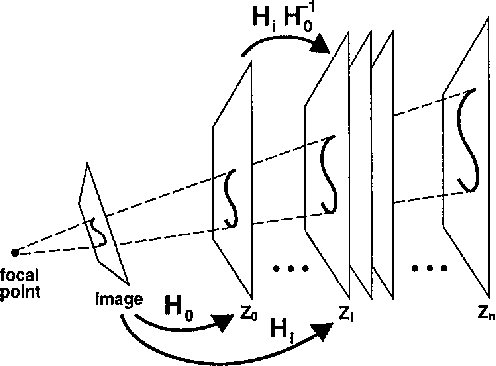
\includegraphics[width=0.5\textwidth]{images/psw.png}
      \caption[Plane sweep operation]{\textbf{Plane sweep operation.} Pixels from each image are back-projected onto successive positions $Z = z_i$ of a plane that sweeps through the camera's frustum with homography $H_i$. $H_0$ is the homography that maps the image points to the plane at $Z = z_0$. By combining the two, we can say that the homography that maps pixels between the planes $Z = z_0$ and $Z = z_i$ directly, by forward projection from the $z_0$ plane onto the image, then back-projection to the $z_i$ plane, can be written as $H_i\inv{H_0}$. This image is taken from \cite{Collins1996ASA}}.
       \label{fig:psw}
\end{figure}
The entire depth range in the reference frustum is discretized. This is a common step in many MVS algorithms and is essential for constructing the cost volume. The depth $d_i$ at the $i^{th}$ plane can be calculated as:
\begin{equation}
    d_i = \mathbf{D_{min}} + i \times \frac{\mathbf{D_{max}-D_{min}}}{N-1} \hspace{0.5cm} \text{for} \hspace{0.5cm} i=0, \dots, N-1
\end{equation}\label{eq:dist-discrete}
Here, $[\mathbf{D_{min}}, \mathbf{D_{max}}]$ is the depth range of the scene. $N$ is the number of depth planes in the cost volume. In the camera's frustum, each of these depth levels corresponds to a "plane" parallel to the image plane of the camera. Then, every pixel in the reference image will have $N$ depth hypotheses corresponding to these $N$ planes. The task of the MVS algorithm will be to determine the most likely depth value for each pixel. Increasing $N$ reduces the discretization errors in the results and increases the number of parameters in the network and, thus, the GPU memory. In this thesis, we use $N=256$ for {\rmvd} and $N=128$ for {\mvsn}.

Once the depth has been discretized, we must align the pixels between the reference and the source images using a homography $\mathbf{x'} ~ \mathbf{H_k}(d_i)\cdot \mathbf{x}$ where $∼$ indicates equality up to scale \cite{Szeliski2010book, Yao2018}.  Only then can we measure the similarity between the reference and the source features. In the depth hypothesis $d_i$, we first project all pixels of a source feature into space with $d_i$ and then back-project these points through the reference camera. Thus using \hyperref[eq:world-to-pix]{Equation 7} and the projection equation from \hyperref[fig:psw]{Figure 2}, the homography between the $k^{th}$ source image and the reference image at depth $d_i$ can be obtained as:
\begin{equation}
    \mathbf{H_k}(d_i)= d_i\mathbf{K_0T_0\inv{T_k}\inv{K_k}}
\end{equation}\label{eq:homography}
where $\mathbf{K_0}$ and $\mathbf{T_0}$ are the camera intrinsics and extrinsics matrices of the reference image. \cite{zhu2021deep}

After the depth discretization and the warping operation, we can now construct a cost volume. This is essentially a 3D volume where one dimension corresponds to the image's width, another to its height, and the third to the depth levels.
Each voxel 3D pixel in this volume corresponds to a pixel in the reference image and a specific depth level. The voxel's value or "cost" represents how well that depth matches the observations from the other images based on some metric. Depth estimation involves finding the depth level with the minimum cost for each pixel and producing a dense depth or disparity map. The methods explored in this thesis use normalized cross-correlation as a similarity metric. \par
One of the baselines {\mvsn} does not employ any correlation but only warps the source features to the reference features and fuses the cost volumes with a variance-based strategy. {\rmvd} uses the Dispnet correlation layer \cite{Mayer2016} that employs the full correlation and decimates the feature dimension. Schröppel \etal in the {\rmvd} framework \cite{schroeppel2022benchmark} improved the plane sweep homography warping described above for the pairwise cost volume construction. This is done by explicitly enforcing the epipolar constraint on the sampling points in the source image before the warping and correlation operations. The sampling points for a point on the reference image are constrained to its epipolar line in the source image at the different depth levels. This reduces the search space for matching points to a 1D search along the epipolar line. As a result of this explicit constraining, the correlation costs are computed between a more accurately warped source and reference image. \hyperref[fig:cvc]{Figure 3} shows the cost volume construction operation in a typical MVS setup. All the models implemented in this thesis use this improved version of the planesweep warping operation. \par
In the next section, we take a look at the complete MVS pipeline and describe in detail each component of the pipeline. 


\section{Multi-view Depth Estimation Pipeline}\label{sec:mvspipeline}
When using deep learning for depth estimation in an MVS setting, the network is typically trained to learn these complex mappings from the input images to the feature maps, cost volumes, and a corresponding depth map guided by a suitable loss function. A common approach involves feeding the network with pairs of images and their corresponding disparity (or depth) maps during the training phase. The network learns to extract features from the images and associate the similarity between the images with the depths. This learned model can be used to predict depth maps from new pairs of images.

One significant advantage of using deep learning for this task is that networks can learn to handle a wide range of complex scenes and lighting conditions, which can be challenging for traditional MVS methods. Moreover, using convolutional layers in these networks allows them to consider the local context in the images, which can significantly improve the accuracy of depth estimation.

An example of a deep learning method for MVS is the MVSNet framework, which uses a differentiable homography warping \cite{Yao2018} layer to aggregate information from multiple views into a cost volume using a variance-based fusion and a 3D CNN to regress the depth map from this cost volume. This framework allows for end-to-end training and can handle an arbitrary number of input views. 

The standard multiview depth estimation pipeline consists of several stages that collectively generate accurate depth maps or point clouds from multiple input images. The main components of this pipeline include a feature encoder, a matching costs computation and aggregation unit, and a component to denoise the aggregated costs known as the regularization unit. The final depth is estimated from the denoised costs. We will dive into each of these components, their different flavors, and the network architectures that use these components as their basis. 

\begin{enumerate}
\item \textbf{Input and Preprocessing:} The input to the pipeline is a set of images of a scene taken from different viewpoints (source views), with one image selected as the reference view. Input images are often preprocessed, including normalization and resizing, to ensure that they are in a suitable format for a neural network. To maintain the integrity of our experiments, we have fixed the input sizes and the sizes of the evaluation data. If a model is trained with smaller inputs due to memory constraints on the GPU, it is explicitly stated. All sizes are multiples of 32. This addresses the size mismatch in spatial dimensions caused by strided convolutional operations on input tensors and skip connections to a layer.

\item \textbf{Feature Extraction:} In this stage, a Convolutional Neural Network (CNN) is used to extract feature maps from input images. The feature extractor scans the images and learns to identify patterns and structures that are important for depth estimation, such as edges, corners, and textures. This process reduces the high-dimensional image data to a more manageable, lower-dimensional form that still contains the information necessary for depth estimation. In this thesis, we examine the feature encoders of MVSNet and DispNet. We also explore the effects of using a multiscale architecture such as a UNet \cite{ronneberger2015unet}  for feature extraction and also look at fusing the learned features with features generated by a pre-trained ViT such as DINO \cite{caron2021emerging}. 

\item \textbf{Cost Volume Construction:} To find correspondences between different views, a cost volume is often constructed. The cost volume effectively represents the likelihood that each pixel in the reference image has a certain depth. We described the construction of a pairwise cost volume using different correlation types and homography warping with the plane sweep algorithm in detail in \hyperref[sec:multiviewster]{Section 2.4} and \hyperref[sec:depthestim]{Section 2.3}. The individual pairwise cost volumes of the reference and source features are fused using different strategies to obtain the aggregated cost volume. The learned fusion involves learning weights for each pairwise cost volume using a 2D or 3D CNN. Views with more occluded points are given less weight in the aggregated cost volume. Average fusion simply fuses all pairwise volumes equally. Variance-based fusion, which is used in {\mvsn} \cite{Yao2018}, compares the variance of the warped source features and the reference feature to fuse the warped volumes. In this thesis, we examine all three fusion strategies. 
\begin{figure}[ht]
\centering
     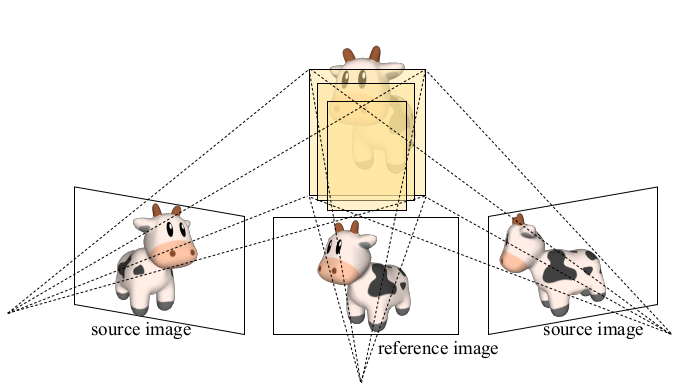
\includegraphics[width=0.75\textwidth]{images/cvc.png}
      \caption[Cost volume construction]{\textbf{Cost volume construction.} Using homography warping with a planesweep volume along the reference camera frustum and computing the matching costs at the different depth planes. This image is taken from \cite{zhu2021deep}.} 
       \label{fig:cvc}
\end{figure}
\item \textbf{Cost Volume Processing and Depth Map Estimation:} The cost volume is typically processed using a 3D CNN \cite{Yao2018, Zhang2020, Gu2020, Yang2020}, or RNN \cite{Yao2019} that aggregates and regularizes information across different views and depths to robustly estimate the depth map of the reference view. This is an essential step due to cost volumes being inherently noisy due to occlusions, poor texture and lighting, and non-Lambertian surfaces. Some techniques use a coarse-to-fine pattern to better estimate the depth and reduce memory consumption. The first level of the network predicts a coarse depth map. This is used as input for subsequent levels to yield finer results. Multiscale feature extractors are used to obtain features at different resolutions. The low-resolution features are used at the coarse level, and the high-resolution features are used as input to the finer levels along with the coarse depth map from the previous level. There are also different implementations of this strategy. Some methods simply use cascade fusion, such as CasMVSNet and CVP-MVSNet\cite{Gu2020, Yang2020} while others, such as Vis-MVSNet \cite{Zhang2020}, also use the uncertainty map to weigh depth residuals. In this thesis, we explore regularization using a regular 2D UNet for {\rmvd} and 3D UNet for {\mvsn}. We also look at cascade warping and implement and experiment with a coarse-to-fine pattern for both these baselines. The coarse-to-fine architecture is shown in \hyperref[fig:ctf]{Figure 4}

\begin{figure}[ht]
\centering
     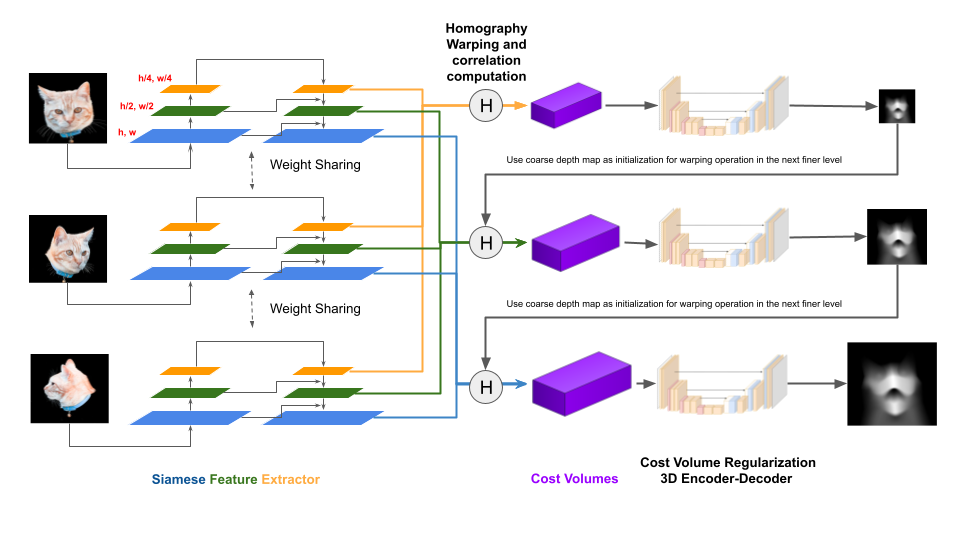
\includegraphics[width=1\textwidth]{images/coarse-to-fine.png}
      \caption[Coarse-to-fine pattern]{\textbf{Coarse-to-fine pattern.} This figure shows a typical coarse-to-fine design. Cost volumes at finer levels are constructed using the coarser depth predictions as initialization. In this figure, a single 3D UNet is used as the regularization network. 3D UNets in a stacked hourglass configuration~\cite{newell2016stacked} are also used to regularize raw cost volumes (in purple). The cost volumes at finer levels have a smaller depth range centered around the previous coarse depth predictions and are coupled with an adaptive subdivision of depth intervals for finer levels. Multilevel features with different spatial resolutions and channel depth are used to construct the cost volumes and depth maps at different levels. A multilevel feature extractor, such as a feature pyramid network or a 2D UNet, can be used for this purpose.}
\label{fig:ctf}
\end{figure}

\item \textbf{Refinement:} The initial depth map from the previous stage is often coarse and may contain inaccuracies. Therefore, it is common to refine the depth map using various methods. This could involve an additional CNN that takes the initial depth map and the reference image as input and learns to predict corrections to the depth values. The network can be trained to minimize the difference between its predictions and ground truth depth maps, if available. In this thesis, we only look at the fundamental elements of the MVS pipeline discussed previously and their interaction. We do not look at the effects of additional image-refinement strategies. 

\item \textbf{Training:} The entire pipeline can be trained from beginning to end using supervised learning, as ground-truth depth maps are available. If not, unsupervised or self-supervised methods can be used, where the training signal comes from photometric consistency or other cues. All experiments in this thesis are performed in a supervised manner, with the correlation between the source and reference images as a signal to guide the entire process. 

\item \textbf{Testing and Evaluation:} Once the pipeline is trained, it can be used to estimate depth maps from new multiview image sets. The datasets used to evaluate and train networks are discussed in detail in \hyperref[sec:datasets]{Section 4.2}. The quality of the depth maps can be evaluated using various metrics, such as mean absolute error or mean squared error, if ground truth is available. The metrics are discussed in \hyperref[sec:metrics]{Section 4.3}. Visual inspection and downstream tasks can also be used for evaluation.

\end{enumerate}\par
There are several versions of this pipeline that are tailored to different tasks, data availability, and current research advancements. Some of the recent approaches suggest the inclusion of transformer architectures, attention mechanisms, and other advanced techniques such as coarse-to-fine architecture, feature pyramids, and pre-trained vision transformers as feature extractors in the pipeline to enhance the accuracy of depth estimation. In the following chapter, we will conduct a comprehensive evaluation of these methodologies.



